\documentclass[t,aspectratio=169]{beamer}

\usepackage{soul}
\usepackage[utf8]{inputenc}

% ----------------------------------------------------------------------------------------------------------------------------------------

\title{
\includegraphics[width=45pt]{oepecsetlogo.png}\\(KTXFI2EBNF) Physics II. Practice}

% \subtitle{1-4. lecture}

\author{Dr.~Gábor FACSKÓ, PhD\\\tiny Assistant Professor / Senior Research Fellow\\\textit{facsko.gabor@uni-obuda.hu}}

\institute{\Tiny Óbuda University, Faculty of Electrical Engineering, 1084 Budapest, Tavaszmező u. 17.\\Wigner Research Centre for Physics, Department of Space Physics and Space Technology, 1121 Budapest, Konkoly-Thege Miklós út 29–33.\\ \url{https://wigner.hu/~facsko.gabor}}

\date{November 24,~2025}

\logo{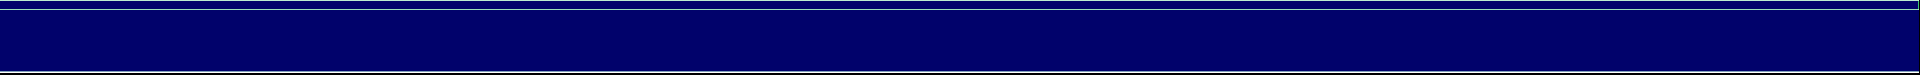
\includegraphics[height=0.9 true cm]{kekcsik.png}}

% ----------------------------------------------------------------------------------------------------------------------------------------

\begin{document}

\frame{\titlepage}

% ----------------------------------------------------------------------------------------------------------------------------------------

\begin{frame}%[fragile,squeeze,allowframebreaks]
\frametitle{Common Business}
\begin{itemize}
\setlength{\parskip}{0pt}
\item Homework 3 will be released soon.
\item The midterm exam scheduled for December 1, 2025 will cover Exercise Groups 1–3, that is, Homework 1–3.
\item We will not have time to work on Exercise Group 4 $\rightarrow$ Homework 4–5 \underline{after} the midterm exam.
\item I will not be present on December 8, 2025, when you will have the opportunity to retake the midterm exam; however, I will provide you with the necessary exercises.
\item I \textbf{must} finalize the grading of your midterm exam before December 8, 2025.
\end{itemize}
\end{frame}

% ----------------------------------------------------------------------------------------------------------------------------------------

\begin{frame}
%\frametitle{Minden jó, ha a vége jó}

\vfill
\begin{center}
\textbf{\huge The End}

\bigskip
Thank you for your attention!
\end{center}
\vfill
\end{frame}

\end{document}
